% (c) Copyright 2017 Josh Wright
\documentclass[12pt]{article}
\usepackage{verbatim}
% \usepackage{syntonly}
\usepackage{ragged2e}
\usepackage{geometry}
\usepackage{enumitem} % for longenum
\usepackage{setspace}
\usepackage{hyperref}
\usepackage{circuitikz}
\usepackage{tabularx}
\usepackage{graphicx}
\usepackage{outlines} % for outline
\usepackage{paralist} % for compactitem (compact itemize)
\usepackage{multicol} % for multicolumn layout
\geometry{letterpaper, margin=0.4in, top=0.2in}
% \geometry{letterpaper, margin=0.5in, top=0.35in, left=1.5in}
\pagenumbering{gobble}
\begin{document}
\begin{spacing}{0.8}
%%%%%%%%%%%%%%%%%%
%% main section %%
%%%%%%%%%%%%%%%%%%
\begin{multicols*}{2}
\begin{flushleft}
\newlist{longenum}{itemize}{5}
\setlist[longenum,1]{nosep,leftmargin=0.2cm,labelwidth=0px,align=left,label=$\bullet$}
\setlist[longenum,2]{nosep,leftmargin=0.2cm,labelwidth=0px,align=left,label=$\ast$}
\setlist[longenum,3]{nosep,leftmargin=0.2cm,labelwidth=0px,align=left,label=\texttt{=}}
\setlist[longenum,4]{nosep,leftmargin=0.2cm,labelwidth=0px,align=left,label=>}
\setlist[longenum,5]{nosep,leftmargin=0.2cm,labelwidth=0px,align=left,label=@}
% \begin{outline}[compactitem]
\begin{outline}[longenum]
%%%%%%%%%%%%%%%%%%%%
%% spacing config %%
%%%%%%%%%%%%%%%%%%%%
% just in case I need even more space
\newlength{\upspacelength}
\setlength{\upspacelength}{0px}
\newcommand{\upspace}{\vspace{\upspacelength}}
% section titles
\newcommand{\zzz}[1]{\upspace \0 \textbf{#1} }
% \newcommand{\zzz}[1]{\0 \hspace{-1.25in} \textbf{#1} \vspace{-10px} }
% makes second-level itemize bullets instead of dashes
% \renewcommand\labelitemii{\labelitemi}
% redefine the sub-headings to inject our space-saver
\let\oldOne\1\let\oldTwo\2\let\oldThree\3\let\oldFour\4
\renewcommand{\1}{\oldOne   \hspace{-8px}}
\renewcommand{\2}{\oldTwo   \hspace{-8px}}
\renewcommand{\3}{\oldThree \hspace{-8px}}
\renewcommand{\4}{\oldFour  \hspace{-8px}}
\small

\noindent ECEN325 Ref Sheet \hfill \textcopyright \space Josh Wright \today

\zzz{Metric Prefixes} \\
\begin{tabular}{|c c l l|}                                   \hline
peta  & P     & $10^{ 15}$ & \hfill 1 000 000 000 000 000 \\ \hline
tera  & T     & $10^{ 12}$ & \hfill     1 000 000 000 000 \\ \hline
giga  & G     & $10^{  9}$ & \hfill         1 000 000 000 \\ \hline
mega  & M     & $10^{  6}$ & \hfill             1 000 000 \\ \hline
kilo  & k     & $10^{  3}$ & \hfill                 1 000 \\ \hline
hecto & h     & $10^{  2}$ & \hfill                   100 \\ \hline
deca  & da    & $10^{  1}$ & \hfill                    10 \\ \hline
one   &       & $10^{ 0 }$ & \hfill       1 \hfill \hfill \\ \hline
deci  & d     & $10^{- 1}$ & 0.1                          \\ \hline
centi & c     & $10^{- 2}$ & 0.01                         \\ \hline
milli & m     & $10^{- 3}$ & 0.001                        \\ \hline
micro & $\mu$ & $10^{- 6}$ & 0.000 001                    \\ \hline
nano  & n     & $10^{- 9}$ & 0.000 000 001                \\ \hline
pico  & p     & $10^{-12}$ & 0.000 000 000 001            \\ \hline
femto & f     & $10^{-15}$ & 0.000 000 000 000 001        \\ \hline
\end{tabular}

\zzz{Ohm's Law}
  $V = IR$,
  \quad $I = \frac{V}{R}$,
  \quad $R = \frac{V}{I}$


\zzz{Complex Numbers}
  \1 $z = x+iy = re^{i\theta} = r[\cos(\theta)+i\sin(\theta)]$
  \1 $[r(\cos(\theta)+i\sin(\theta))]^n = r^n[\cos(n\theta)+i\sin(n\theta)]$
  \1 $z^n = (re^{i\theta}) = r^ne^{in\theta}$
  \1 $\frac{1}{i}=-i$
  \1 $\sqrt[n]{z} = \sqrt[n]{r}e^{\frac{\theta}{n}+\frac{2k\pi}{n}}$ for $n\in N^*$ (ints $\geq0$)
  \1 $e^{j\theta} = \cos(\theta) + j\sin(\theta)$
  \1 $e^{-j\theta} = \cos(\theta) - j\sin(\theta)$
  \1 $\cos(\theta) = \frac{1}{2}(e^{j\theta} + e^{-j\theta})$
  \1 $\sin(\theta) = \frac{1}{2j}(e^{j\theta} - e^{-j\theta})$
  \1 normalized: $sinc(t) = \frac{\sin(\pi t)}{\pi t}$
  \1 $|\frac{a}{b}| = \frac{|a|}{|b|}$
  \1 $\angle\frac{a}{b} = \angle{a} - \angle{b}$

\zzz{Trig}
  \1 $\cos^2(a)+\sin^2(a)=1$
  \1 $\cos(2a)=\cos^2(a) - \sin^2(a) = 2\cos^2(a)-1 = 1-2\sin^2(a)$
  \1 $\sin(2a) = 2\sin(a)\cos(a)$
  \1 $\cos^2(a) = \frac{1}{2}(1 + \cos(2a))$
  \1 $\sin^2(a) = \frac{1}{2}(1 - \cos(2a))$


% \zzz{RC Filter}
%   \1 Transmission Function: $T(s) = \frac{V_o(s)}{V_i(s)}$
%   \1 Corner frequency: frequency $s$ at which $T(s)=\frac{1}{\sqrt{2}}$
%   \1 for simple circuit:
%     ground$\rightarrow$source$\rightarrow R \rightarrow C\rightarrow$ground
%     \2 $T(s)=\frac{1}{1+RCs}$
%     \\ $|T(j\omega)|=\frac{1}{\sqrt{1+R^2C^2s^2}}$
%     \\ $|\angle T(j\omega)|=\frac{1}{\sqrt{1+R^2C^2s^2}}$
%   \1 low pass
%     \2\begin{circuitikz}
%       \draw
%       (0,3) to [short, o-,l=$V_i$] (0,3)
%       (0,3) to [R, -*, l=$R$] (3,3)
%       (3,3) to [C, -, l=$C$] (3,2)
%       (3,2) to node[ground]{} (3,2)
%       (3,3) to [short, -o,l=$V_o$] (4,3);
%       \end{circuitikz}
%     \2 $T(s)=\frac{V_o}{V_i}=\frac{1}{1 + RCs}$
%     \2 corner frequency: $s=\frac{1}{RC}$ (also pole)
%     \2 pole: $\frac{1}{RC}$
%   \1 high pass
%     \2\begin{circuitikz}
%       \draw
%       (0,3) to [short, o-,l=$V_i$] (0,3)
%       (0,3) to [C, -*, l=$C$] (3,3)
%       (3,3) to [R, -, l=$R$] (3,1)
%       (3,1) to node[ground]{} (3,1.5)
%       (3,3) to [short, -o,l=$V_o$] (4,3);
%       \end{circuitikz}
%     \2 $T(s)=\frac{V_o}{V_i}=\frac{RCs}{1+RCs}$
%     \2 zero: $s=0$, pole: $s=\frac{1}{RC}$
% 
% \zzz{Bode Plots}
%   \1 magnitude is plotted in $dB$: $|T(j\omega)|_{dB}=20\log_{10}|T(j\omega)|$
%   \1 starts on y-axis at DC offset with slope 0
%   \1 just add together the bode plots of each individual pole, zero, and the DC offset
%   \1 poles always slope down, zeros slope up
%     \\ (applies for both magnitude and phase)
%   \1 $dec$=decade, e.g. from $10^0$ to $10^1$
%   \1 magnitude:
%     \2 Pole/Zero at origin:
%       \\ constant slope $\pm20db/dec$ for all $\omega$; $0dB$ at $\omega=10^0=1$
%     \2 Pole/Zero at $\omega_0$:
%       \\ 0 for $\omega<\omega_0$
%       \\ slope $\pm20\frac{db}{dec}$ after
%     \2 Constant $C$: constant line at $20\log_{10}(|C|)$
%   \1 phase:
%     \2 Pole at origin: constant $-\frac{\pi}{2}$ or $-90^\circ$
%     \2 Zero at origin: constant $+\frac{\pi}{2}$ or $+90^\circ$
%     \2 Pole/Zero at $\omega_0$:
%       \\ $0$ for $\omega<\frac{\omega_0}{10}$
%       \\ slope linearly ($\pm45^\circ/dec$) until $10\omega_0$
%       \\ $0$ slope for $\omega>10\omega_0$
%     \2 Constant $C$: no effect ($0$ for all $\omega$)
%   \1 Prof wants us to actually show the -3dB drop curve, not just a straight intersection
% 
% \zzz{Solving systems with Op Amps}
%     \1 step 0: if the op amp is ideal, write out ideal properties:
%         \2 $V_+=V_-$
%         \2 $I_-=0,I_+=0$
%     \2 $A \approx \infty$
%     \1 avoid doing KCL/KVL directly on the output node of the op amp
%     \1 ignore resistors from a point at $0V$ to ground
% 
% \zzz{Non-Ideal Op Amps}
%   \1 still assume that current at input terminals is 0
%   \1 $V_o = A (V_{+} - V_{-})$
%     \2 $A$: open-loop gain. Typically very large, 100,000 or more
%   \1 open-loop gain dependent on frequency: $A(s)=\frac{A_0}{1-\frac{s}{\omega_b}}$
%     \2 open-loop response drops off after $\omega_b$
%       \\(usually $2\pi \leq \omega_b \leq 2\pi100$)
%     \2 $A_0$: DC gain
%     \2 $\omega_t$: unity gain frequency: $dB(T(\omega_t))=1$
%       \\ $\omega_t \approx A_o \omega_b$
%       \\ AKA gain bandwidth product
%     \2 in this case, we still assume $I_-=I_+=0$ and $V_-=V_+$?
%   \1 slew rate
%     \2 max rate at which the output can change
%     \2 for a sinusoidal signal: ($V_{pk}$: peak voltage)
%       \\ $SR > 2 \pi f V_{pk}$ or $SR > \omega V_{pk}$
%       \\ $\frac{dV_o}{dt}|_{MAX} < SR$
% 
% 
% 
% \zzz{Op Amp Equations}
%   % http://pdp7.org/synthwiki/OpAmpCircuits.html
%   \1 general form: $T(s)=\frac{K_0}{1+\frac{s}{\omega_0}}$
%     \2 $T(0)=K_0$: DC offset. For these simple ones, it's equal to ideal response
%     \2 $\omega_0=\frac{\omega_t}{1+R_2/R_1}$
%   \1 inverting op amp:
%     \2 ideal: $T(s)=\frac{V_o}{V_i}=-\frac{R_2}{R_1}$
%     \2 non-ideal: $T(s)=\frac{V_o}{V_i}
%       =\frac{-R_2/R_1}{1+\frac{1+R_2/R_1}{A(s)}}
%       =\frac{-R_2/R_1}{1+\frac{s}{\left(\frac{\omega_t}{1+R_2/R_1}\right)}}
%       =\frac{-R_2/R_1}{1+\frac{s}{\omega_0}}$
%     \\\begin{circuitikz}
%       \draw
%       (5,2) node[op amp] (opamp) {}
%       (1,2.5) to [short, o-, l=$V_i$] (1,2.5)
%       (1,2.5) to [R, l=$R_1$] (opamp.-)
%       (3.8,3.5) to [R, l=$R_2$] (6.2,3.5)
%       (opamp.+) to (3.8,1.2) node[ground]{}
%       (3.8,3.5) to [short, -*] (opamp.-)
%       (6.2,3.5) to [short, -*] (opamp.out)
%       (opamp.out) to [short, -o, l=$V_o$] (7, 2);
%       \end{circuitikz}
%   \1 non-inverting op-amp:
%     \2 ideal: $T(s)=\frac{V_o}{V_i}=1+\frac{R_2}{R_1}$
%     \2 non-ideal: $T(s)=\frac{V_o}{V_i}
%       =\frac{1+R_2/R_1}{1+\frac{1+R_2/R_1}{A(s)}}
%       =\frac{1+R_2/R_1}{1+\frac{s}{\left(\frac{\omega_t}{1+R_2/R_1}\right)}}
%       =\frac{1+R_2/R_1}{1+\frac{s}{\omega_0}}$
%     \\\begin{circuitikz}
%       \draw
%       (5,2) node[op amp] (opamp) {}
%       (1,2.5) to [short, -] (1,2) node[ground]{}
%       (1,2.5) to [R, l=$R_1$] (opamp.-)
%       (3.8,3.5) to [R, l=$R_2$] (6.2,3.5)
%       (opamp.+) to (3.5,1.5)
%       (3.5,1.5) to [short, o-, l=$V_i$] (3.5,1.5)
%       (3.8,3.5) to [short, -*] (opamp.-)
%       (6.2,3.5) to [short, -*] (opamp.out)
%       (opamp.out) to [short, -o, l=$V_o$] (7, 2);
%       \end{circuitikz}
%   \1 integrating
%     \2 ideal: $V_o = -\int_{0}^{t} \frac{V_i}{RC} dt + C$
%       \3 $C=$ $V_o(t)$ at $t=0$
%     \\\begin{circuitikz}
%       \draw
%       (5,2) node[op amp] (opamp) {}
%       (0,2.5) to [C, l=$C$] (opamp.-)
%       (0,2.5) to [short, o-] (0,2.5)
%       (3.8,1.25) node[ground]{} to [short, -] (opamp.+)
%       (3.8,3.5) to [R, l=$R$] (6.2,3.5)
%       (3.8,3.5) to [short, -*] (opamp.-)
%       (6.2,3.5) to [short, -*] (opamp.out)
%       (0,2.5) to [short, o-, l=$V_i$] (0,2.5)
%       (opamp.out) to [short, -o, l=$V_o$] (7,2);
%       \end{circuitikz}
%   \1 differentiating
%     \2 ideal: $V_o = -RC \frac{dV_i}{dt}$
%     \\\begin{circuitikz}
%       \draw
%       (5,2) node[op amp] (opamp) {}
%       (0,2.5) to [R, l=$R$] (opamp.-)
%       (0,2.5) to [short, o-] (0,2.5)
%       (3.8,1.25) node[ground]{} to [short, -] (opamp.+)
%       (3.8,3.5) to [C, l=$C$] (6.2,3.5)
%       (3.8,3.5) to [short, -*] (opamp.-)
%       (6.2,3.5) to [short, -*] (opamp.out)
%       (0,2.5) to [short, o-, l=$V_i$] (0,2.5)
%       (opamp.out) to [short, -o, l=$V_o$] (7,2);
%       \end{circuitikz}
%   \1 summing
%     \2 ideal: $V_o = -R_f\left(\frac{V_1}{R_1} + \frac{V_2}{R_2}\right)$
%     \\\begin{circuitikz}
%       \draw
%       (5,2) node[op amp] (opamp) {}
%       (1,3.5) to [R,l=$R_{1}$] (3, 3.5)
%       (0,2.5) to [R,l_=$R_{2}$] (opamp.-)
%       (3,3.5) to [short,-*] (3,2.5)
%       (0,2.5) to [short, o-,l=$V_2$] (1,2.5)
%       (0,3.5) to [short, o-,l=$V_1$] (1,3.5)
%       (3.8,3.5) to [R, l=$R_{f}$] (6.2,3.5)
%       (3.8,3.5) to [short, -*] (opamp.-)
%       (6.2,3.5) to [short, -*] (opamp.out)
%       (opamp.out) to [short, -o, l=$V_o$] (7,2)
%       (3.8,1.25) node[ground]{} to [short, -] (opamp.+);
%       \end{circuitikz}
%   \1 differential (subtracting)
%     \2 ideal: $V_o = \frac{(R_f + R_1) R_g}{(R_g + R_2) R_1} V_2 - \frac{R_f}{R_1} V_1$
%     \\\begin{circuitikz}
%       \draw
%       (4,4) node[op amp] (opamp) {}
%       (0,3.5) to [short, o-,l=$V_2$] (1,3.5)
%       (0,4.5) to [short, o-,l=$V_1$] (1,4.5)
%       (1,4.5) to [R, l=$R_1$] (2.5,4.5)
%       (2.5,4.5) to [short,-*] (2.8,4.5)
%       (2.8,3.5) to [R, l=$R_g$] (2.8,2) node[ground]{}
%       (2.8,3.5) to [short,*-*] (2.8,3.5)
%       (1,3.5) to [R,l_=$R_2$] (2.5,3.5)
%       (2.5,3.5) -- (opamp.+) (3.2,5.5) to [R, l=$R_f$] (5.2,5.5)
%       (5.2,5.5) to [short,-*] (opamp.out) (4.8,4) to [short,-o] (6,4)
%       (opamp.out) to [short,-o, l=$V_o$] (6,4)
%       (opamp.-) -- (2.8,5.5)
%       (2.8,5.5) -- (2.8,5.5) -- (3.2,5.5);
%       \end{circuitikz}

% move the diode symbol over to the right side and up
\zzz{Diodes}
\\\vspace{-40px}
\hfill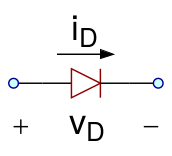
\includegraphics[width=0.25\columnwidth]{../ecen325/diode.png}
\vspace{-20px}
  \1 ideal:
    \2 $I_D(V_D <    0) = 0$
    \2 $I_D(V_D \geq 0) = \infty$
  \1 constant drop model: (just the ideal model shifted right by 0.7V)
    \2 $I_D(V_D <    0.7) = 0$
    \2 $I_D(V_D \geq 0.7) = \infty$
  \1 exponential model: $I_D = I_S ( e^{\frac{V_D}{n V_T}} - 1 )$
    \2 $I_S=10^{-12}$A (saturation current)
    \2 $V_T=25$mV
  \1 small signal resistance: $R_d = \frac{nV_T}{I_D}$
    \2 $I_D$: average (DC) current through diode (due to forward bias)
  \1 bridge rectifier shape: square/diamond with all the diodes point toward the + end of the output (away from ground)
  \\ current goes $\rightarrow$ from cathode (-) to anode (+)

\zzz{Design an (unregulated) AC adapter}
  \1 $V_S$: AC voltage input
    \2 standard AC voltage is $110\sqrt{2}V \approx155.563V$
  \1 $V_{S2}$: output of transformer (still AC)
  \1 $V_p$: peak DC output
  \2 $V_r$: peak-to-peak ripple voltage (maximum variation)
  \1 $V_p=V_{S2}-$ (diode voltage)
    \2 diode voltage = 0.7V for single wave rectifier or center-tapped transformer
    \2 diode voltage = 1.4V for full-wave rectifier
    \2 (corresponds to how many diodes you need)
  \1 turns ratio = $n=\frac{V_S}{V_{S2}}$
  \1 apparent load resistance: $R_L = \frac{V_o}{I_L}$
  \1 ripple voltage: $V_r=\frac{f}{R_L C}$
    \2 $f$: actual ripple frequency (double for full-wave rectifier)
    \2 $C$: filter cap size
  \1 Peak Inverse Voltage: $ PIV = V_{S2}-0.7V$
  \1 avg diode current: $I_{Davg}=I_L \left( 1+\pi\sqrt{\frac{2}{V_r}} \right)$
  \1 max diode current: $I_{Dmax}=I_L \left( 1+2\pi\sqrt{\frac{2}{V_r}} \right)$
    \2 only difference is $\pi \rightarrow 2\pi$

\zzz{Transistors}
  \1 $V_T = 25$mV at room temperature (according to textbook and prof),
  \\ $V_T = 26$mV at room temperature (according to lab)
  \1 $\beta$: a physical constant of the transistor. Usually about 100 or 200
  \1 
    $I_B + I_C = I_E$, 
    $I_C = \beta I_B$,
    $I_E = (1+\beta) I_B$
  \1
    $\alpha = \frac{\beta}{1+\beta}$,
    $I_C = \alpha I_E$
  \1
    $I_C = I_S ( e^{\frac{V_{BE}}{n V_T}} )$,
  \1 AC (assumes correct DC bias):
    $g_m = \frac{1}{r_e} = \frac{I_C}{V_T}$

\zzz{Current Mirror}\\
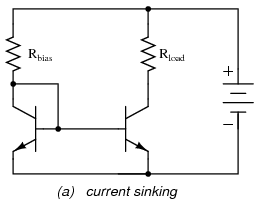
\includegraphics[width=0.46\columnwidth]{../ecen325/current_mirror_npn.png}
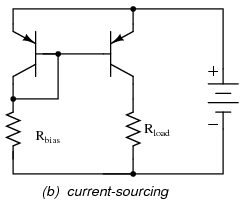
\includegraphics[width=0.44\columnwidth]{../ecen325/current_mirror_pnp.png}
  \1 Q1 has the base shorted to collector, Q2 does not
  \1 $R_{bias}=R_{ref}$: the current that is mirrored
  \1 $I_{ref}=(V_{CC}-0.7)/R_{ref}$
  \1 $R_{load}$ has the same current through it as $R_{ref}$ does
    \2 that is, $I_{ref} = I_{load}$
  \1 you can chain together multiple transistors (Q3,Q4...) all off of
    the same Q1 and they will all get the same current
    \2 In this case, each Q2,Q3... output is considered separate from each other
      in both DC and AC analysis
  \1 only applies when transistors are matched! (we assume they are)

\zzz{Transistor circuits by inspection}
  \1 this all assumes that the transistor is properly DC biased
  \1 three types of amplifier circuits: common emitter, common base, common collector
    \2 CE, CB, CC
    \2 the ``common'' pin is the one that is neither AC input nor output
  \1 intrinsic gain: gain directly from the input pin of the transistor to the output, ignoring any source resistance or such things whatever
    \2 when you chain multiple amplifiers together, this is the one you use
  \1 when you're driving a finite-impedance load (a load other than open circuit), you have to consider $R_o$ as $R_o||R_L$
    \2 this will change the gain, which is why it's often helpful to put a CC buffer at the end of an amplifier
  \1 $R_i$: input impedance: impedance as seen from the input
    \2 includes the transistor, does not include $R_s$
  \1 $g_m = \frac{I_C}{V_T}$
  \\ $r_\pi = \frac{beta}{g_m}$
  \\ $r_e = \frac{V_T}{I_E} = \frac{\alpha}{g_m} \approx \frac{1}{g_m}$
  \\ $r_o = \frac{V_A}{I_C} \approx \infty$
\0
\begin{minipage}{0.3\columnwidth}
  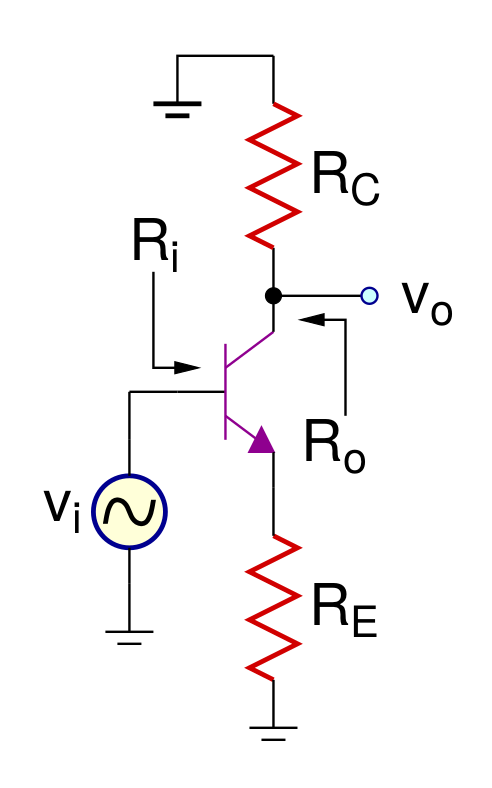
\includegraphics[width=\columnwidth]{../ecen325/bjt_ce.png}
\begin{center}
\vspace{-20px}
{\footnotesize Common Emitter (CE) }
\end{center}
\end{minipage}
\begin{minipage}{0.3\columnwidth}
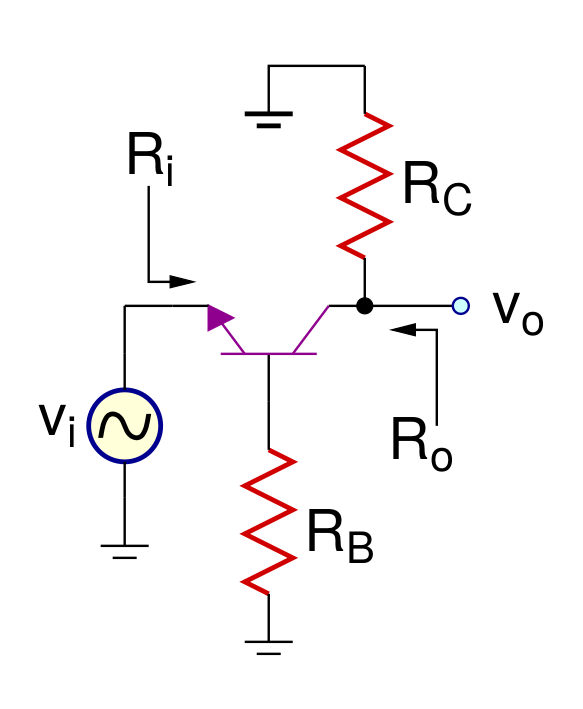
\includegraphics[width=\columnwidth]{../ecen325/bjt_cb.png}
\begin{center} 
{\footnotesize Common Base (CB) }
\end{center}
\end{minipage}
\begin{minipage}{0.3\columnwidth}
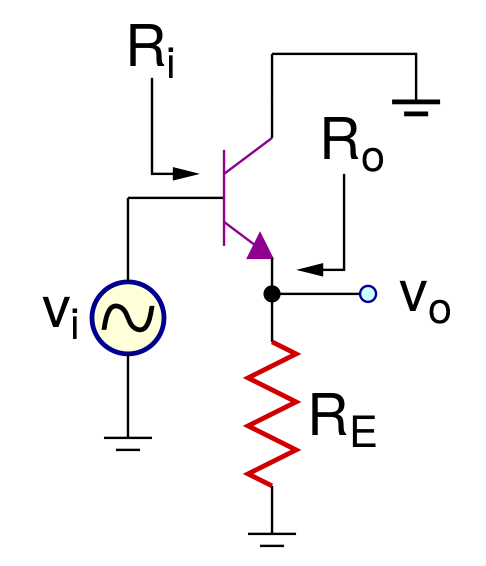
\includegraphics[width=\columnwidth]{../ecen325/bjt_cc.png}
\begin{center} 
{\footnotesize Common Collector (CC) }
\end{center}
\end{minipage}
  \1 CE: Common Emitter
    \2 input: base; output: collector
    \2 intrinsic gain: $\frac{V_o}{V_b}= -\alpha\frac{R_C}{r_e + R_E} \approx -\frac{R_C}{r_e + R_E}$
    \2 $R_i=(\beta+1)(r_e+R_E)$
    \2 $R_o = R_C$
    \2 if you have a $R_L$ then you have to put that in parallel with $R_C$ when calculating $\frac{V_o}{V_b}$
  \1 CB: Common Base
    \2 $\frac{V_o}{V_b} = \alpha\frac{R_C}{R_i} \approx \frac{R_C}{R_i}$
    \2 $R_i = r_e + \frac{R_B}{\beta+1}$
    \2 $R_o=R_C$
  \1 CC: Common Collector
    \2 gain $\approx 1$ because it's a buffer
    \2 $\frac{V_o}{V_b} = \frac{R_E}{r_e+R_E}$
    \2 $R_i = (\beta+1)(r_e+R_E)$
    \2 $R_o = R_E||r_e = \frac{R_E*r_e}{R_E+r_e}$




\end{outline}
\end{flushleft}
\end{multicols*}
\end{spacing}
\end{document}
